\documentclass{article}

\usepackage{neurips_2026}

\usepackage[utf8]{inputenc}
\usepackage[T1]{fontenc}
\usepackage{hyperref}
\usepackage{url}
\usepackage{booktabs}
\usepackage{amsfonts}
\usepackage{amsmath}
\usepackage{amssymb}
\usepackage{amsthm}
\usepackage{nicefrac}
\usepackage{microtype}
\usepackage{xcolor}
\usepackage{algorithm}
\usepackage{algorithmic}
\usepackage{multirow}
\usepackage{graphicx}
\usepackage{subcaption}
\usepackage{pifont}
\usepackage{caption}
\usepackage{bbm}
\usepackage{colortbl}

% Theorem environments
\newtheorem{theorem}{Theorem}
\newtheorem{proposition}[theorem]{Proposition}
\newtheorem{lemma}[theorem]{Lemma}
\newtheorem{corollary}[theorem]{Corollary}
\newtheorem{definition}[theorem]{Definition}
\newtheorem{remark}{Remark}

% Custom commands
\newcommand{\Wbase}{W_0}
\newcommand{\Aseq}{A_{\mathrm{s}}}
\newcommand{\Bseq}{B_{\mathrm{s}}}
\newcommand{\Apar}{A_{\mathrm{p}}}
\newcommand{\Bpar}{B_{\mathrm{p}}}
\newcommand{\Tswitch}{T_{\mathrm{sw}}}
\newcommand{\RR}{\mathbb{R}}
\newcommand{\jelly}{\textsc{Jelly}}
\DeclareMathOperator{\rank}{rank}
\DeclareMathOperator{\diag}{diag}
\DeclareMathOperator{\tr}{tr}

\title{\jelly{}: Generalizing Parameter-Efficient Fine-Tuning\\over the Time Axis via Task-Isomorphic Projection}

\author{Anonymous Author(s)}

\begin{document}

\maketitle

%=============================================================================
\begin{abstract}
%=============================================================================
Parameter-efficient fine-tuning (PEFT) methods such as LoRA fix the adapter topology to a \emph{parallel} connection, bypassing the pretrained weight manifold ($\Wbase$) that sequential adapters exploit for task adaptation.
SVD-based initialization methods (e.g., PiSSA) attempt to utilize $\Wbase$ but require $O(d^3)$ decomposition and remain task-agnostic.
We introduce \jelly{}, a PEFT framework that unifies sequential and parallel adaptations along the training time axis.
During an initial sequential phase, \jelly{} projects activations through $\Wbase$ ($\Wbase x$) to identify the task-intrinsic subspace from data.
At a switching step $\Tswitch$, a lossless \emph{Task-Isomorphic Projection} converts the learned sequential representations into an equivalent parallel adapter via a lightweight double SVD.
This costs $O(dr^2)$---orders of magnitude below full-weight SVD---while preserving the zero additional latency property of LoRA at inference.
Standard LoRA is recovered as the special case $\Tswitch = 0$.
Experiments on LLaMA-2-7B, Mistral-7B, Gemma-7B, and DeBERTa-v3-base across mathematical reasoning (GSM8K, MATH), code generation (HumanEval, MBPP), conversation (MT-Bench), and seven GLUE tasks show that \jelly{} consistently outperforms LoRA, PiSSA, and DoRA, achieving the best score on 6 out of 7 NLU tasks, the highest MATH accuracy on all three NLG base models, and the highest MBPP pass@1 across LLaMA-2-7B, Mistral-7B, and Gemma-7B.
We also show that $\Tswitch$ serves as a geometric indicator of the alignment between the target task and the pretrained manifold.
\end{abstract}
%=============================================================================
\section{Introduction}
\label{sec:intro}
%=============================================================================

Large language models (LLMs) with billions of parameters~\citep{brown2020gpt3, touvron2023llama2} have become the \emph{de facto} foundation for natural language processing and reasoning tasks.
Full fine-tuning of these models is expensive in compute and memory, motivating parameter-efficient fine-tuning (PEFT) methods that update only a small fraction of parameters while keeping the pretrained weights frozen~\citep{lialin2023scaling}.

Among PEFT methods, Low-Rank Adaptation (LoRA)~\citep{hu2022lora} has emerged as the dominant paradigm.
LoRA injects trainable low-rank matrices $B \in \mathbb{R}^{d \times r}$ and $A \in \mathbb{R}^{r \times d}$ in \emph{parallel} with each frozen weight $\Wbase$, yielding the forward pass $h = \Wbase x + BAx$.\footnote{For notational simplicity in the introduction, we assume $d_{\mathrm{in}} = d_{\mathrm{out}} = d$. The general case is treated in Section~\ref{sec:method}.}
The adapter can be reparameterized into $\Wbase$ after training, guaranteeing \emph{zero additional inference latency}.
However, LoRA's random initialization means the early optimization steps operate in a subspace disconnected from the pretrained representations of $\Wbase$, leading to slow initial convergence.

To mitigate this, PiSSA~\citep{meng2024pissa} initializes $B$ and $A$ using the principal singular vectors of $\Wbase$.
While SVD-based initialization accelerates convergence, it requires a full SVD over every target weight matrix at $O(d^3)$ cost per layer.
Because this decomposition is performed before observing any data, it captures the structure of $\Wbase$ but remains \emph{task-agnostic}.

The earliest PEFT methods employed a \emph{sequential} topology~\citep{houlsby2019parameter}, where the adapter processes the output of the base layer: $h = \Wbase x + BA(\Wbase x)$.
This structure uses the feature space of $\Wbase$ as an implicit prior, projecting activations through the pretrained manifold before adaptation.
Sequential adapters were abandoned in favor of parallel methods because they incur inference latency proportional to the model's depth.

We challenge the assumption that sequential and parallel topologies must be mutually exclusive.
We introduce \jelly{} (\textbf{J}oint \textbf{E}fficient \textbf{L}earning with \textbf{L}ayer-\textbf{Y}ielding), a framework that \emph{generalizes} adapter connectivity over the training time axis.
\jelly{} combines the optimization benefits of sequential probing with the inference efficiency of parallel adaptation. Our contributions:

\begin{itemize}
    \item[\bf C1.] \textbf{Time-Axis Generalization.} We formulate adapter connectivity as a function of training progress, transitioning from sequential to parallel at a switching point $\Tswitch \in [0, 1]$. LoRA is recovered as $\Tswitch = 0$.
    \item[\bf C2.] \textbf{Task-Aware Probing.} The sequential phase probes the pretrained manifold from data, identifying the task-intrinsic subspace before parallel training begins.
    \item[\bf C3.] \textbf{$O(dr^2)$ Projection.} A rank-$r$ double SVD converts sequential adapters into equivalent parallel adapters, reducing PiSSA's $O(d^3)$ initialization cost by up to $10^6\times$.
    \item[\bf C4.] \textbf{Zero Inference Overhead.} After projection, training continues in standard LoRA topology with no additional latency at inference.
\end{itemize}

\begin{figure*}[t]
\centering
% Top row: (a) left | (b) right
\begin{subfigure}[b]{0.37\textwidth}
    \centering
    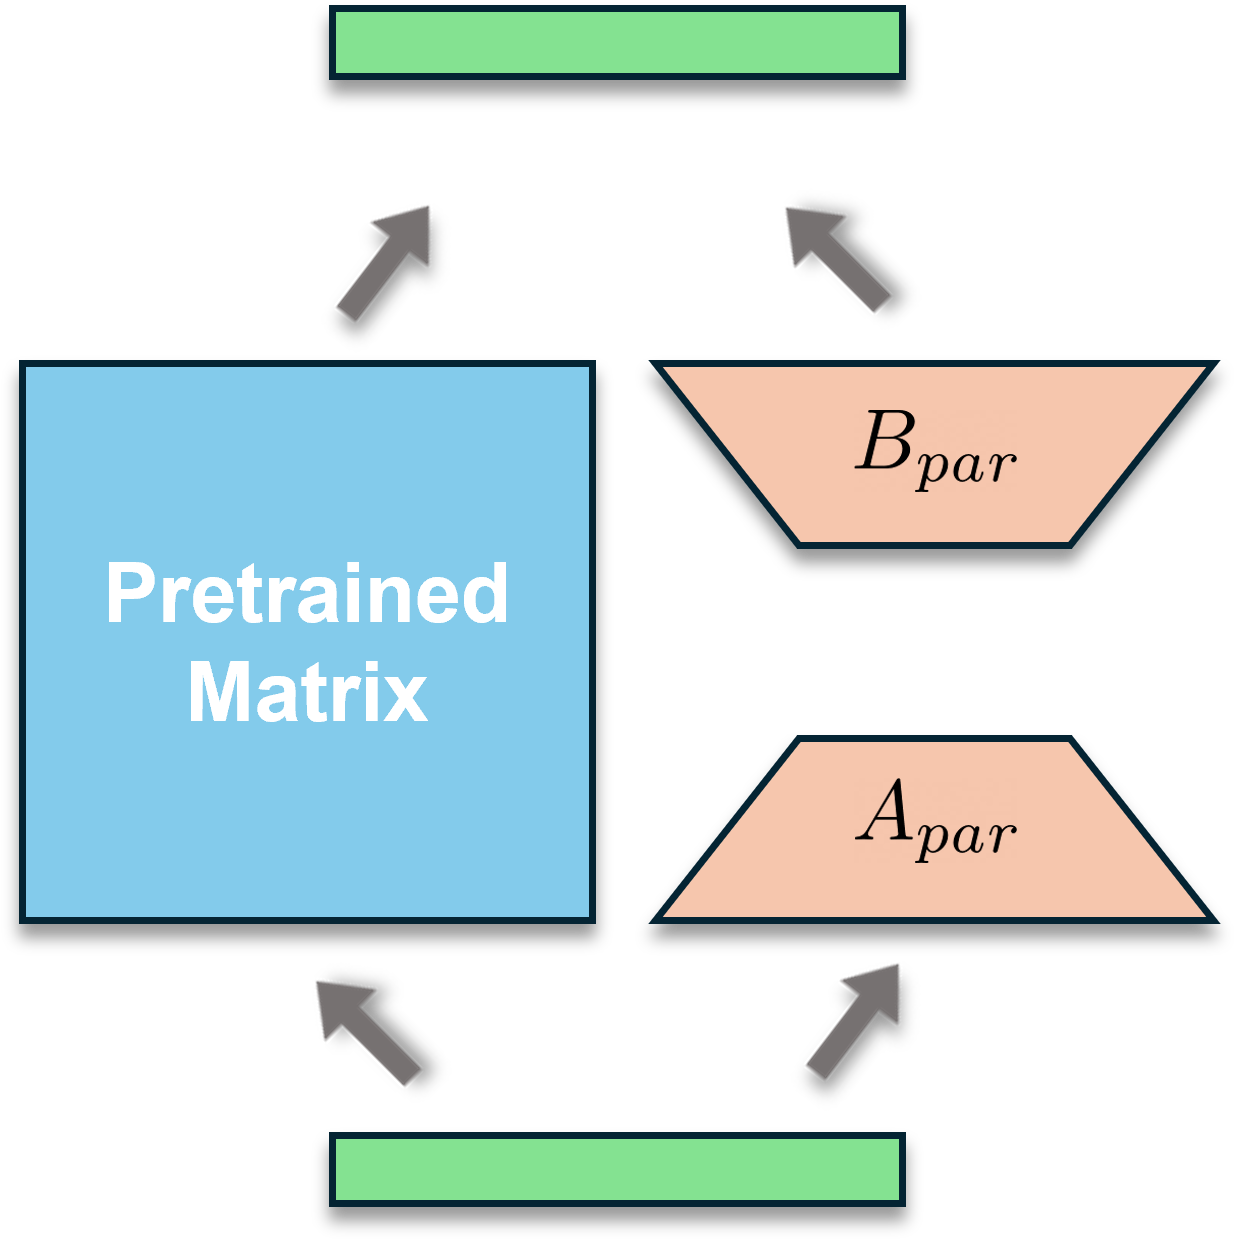
\includegraphics[width=\textwidth]{figures/fig1a.png}
    \caption{Parallel (LoRA)}
    \label{fig:arch_parallel}
\end{subfigure}
\hfill
\vrule width 0.4pt
\hfill
\begin{subfigure}[b]{0.57\textwidth}
    \centering
    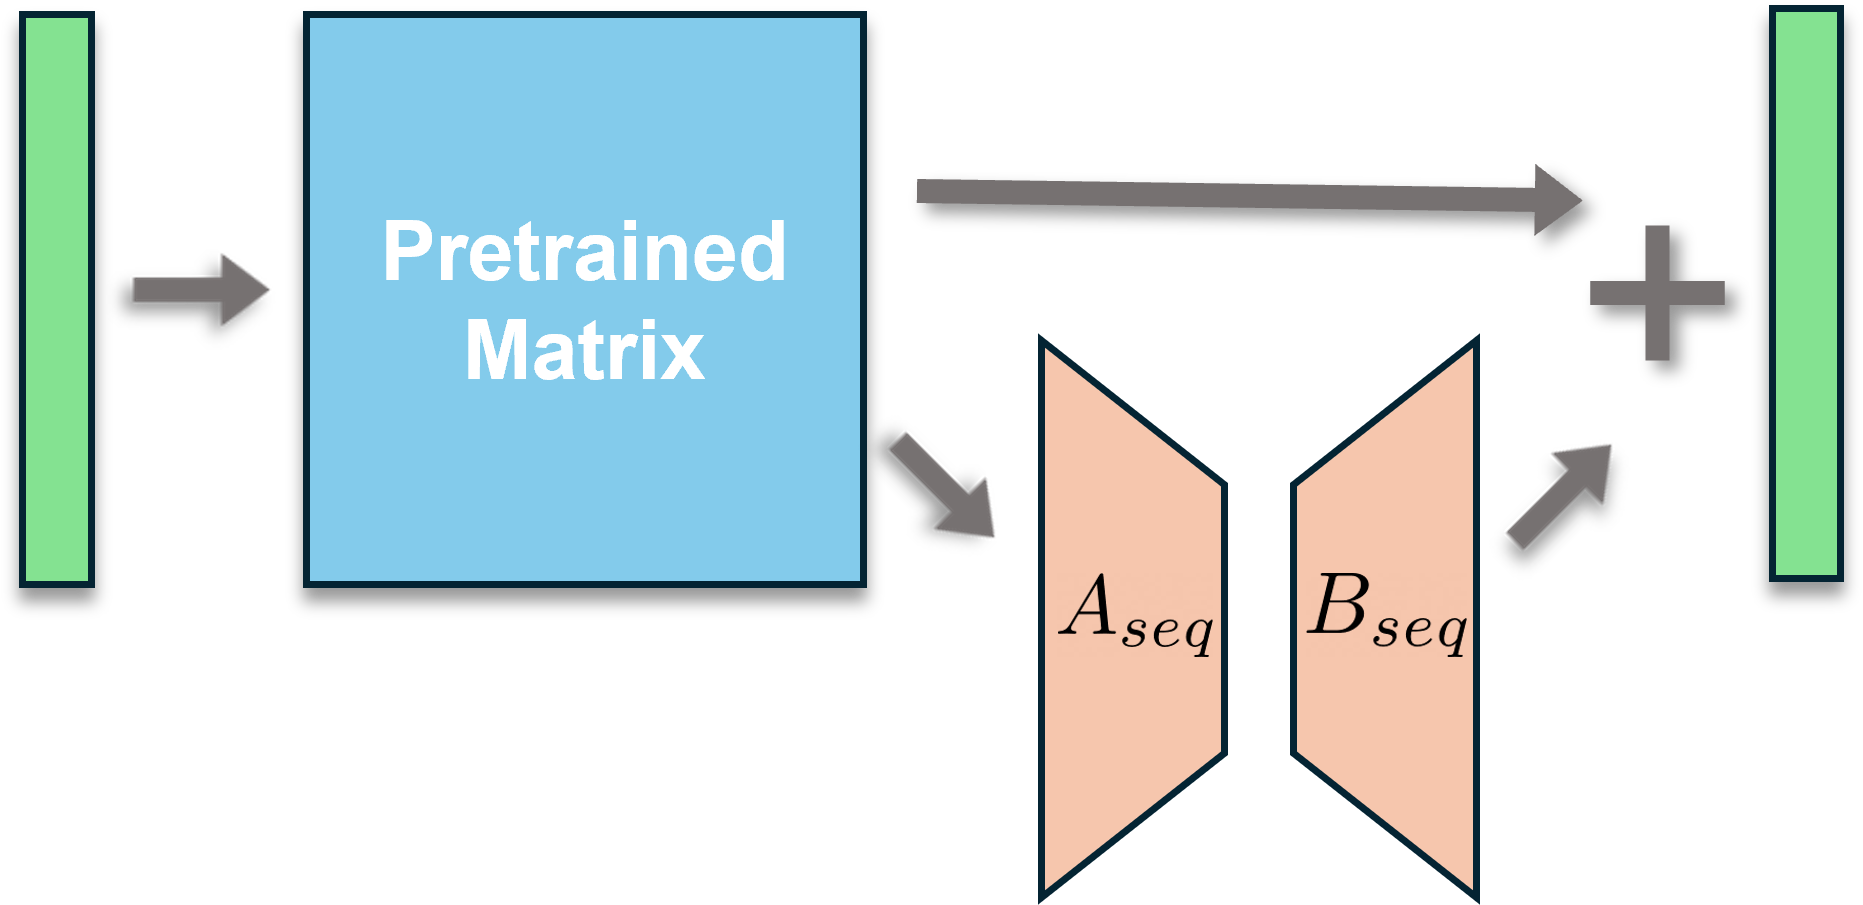
\includegraphics[width=\textwidth]{figures/fig1b.png}
    \caption{Sequential (Houlsby)}
    \label{fig:arch_sequential}
\end{subfigure}
\par\vspace{0.3em}
\noindent\rule{\textwidth}{0.4pt}
\vspace{0.3em}
% Bottom row: (c) full width
\begin{subfigure}[b]{\textwidth}
    \centering
    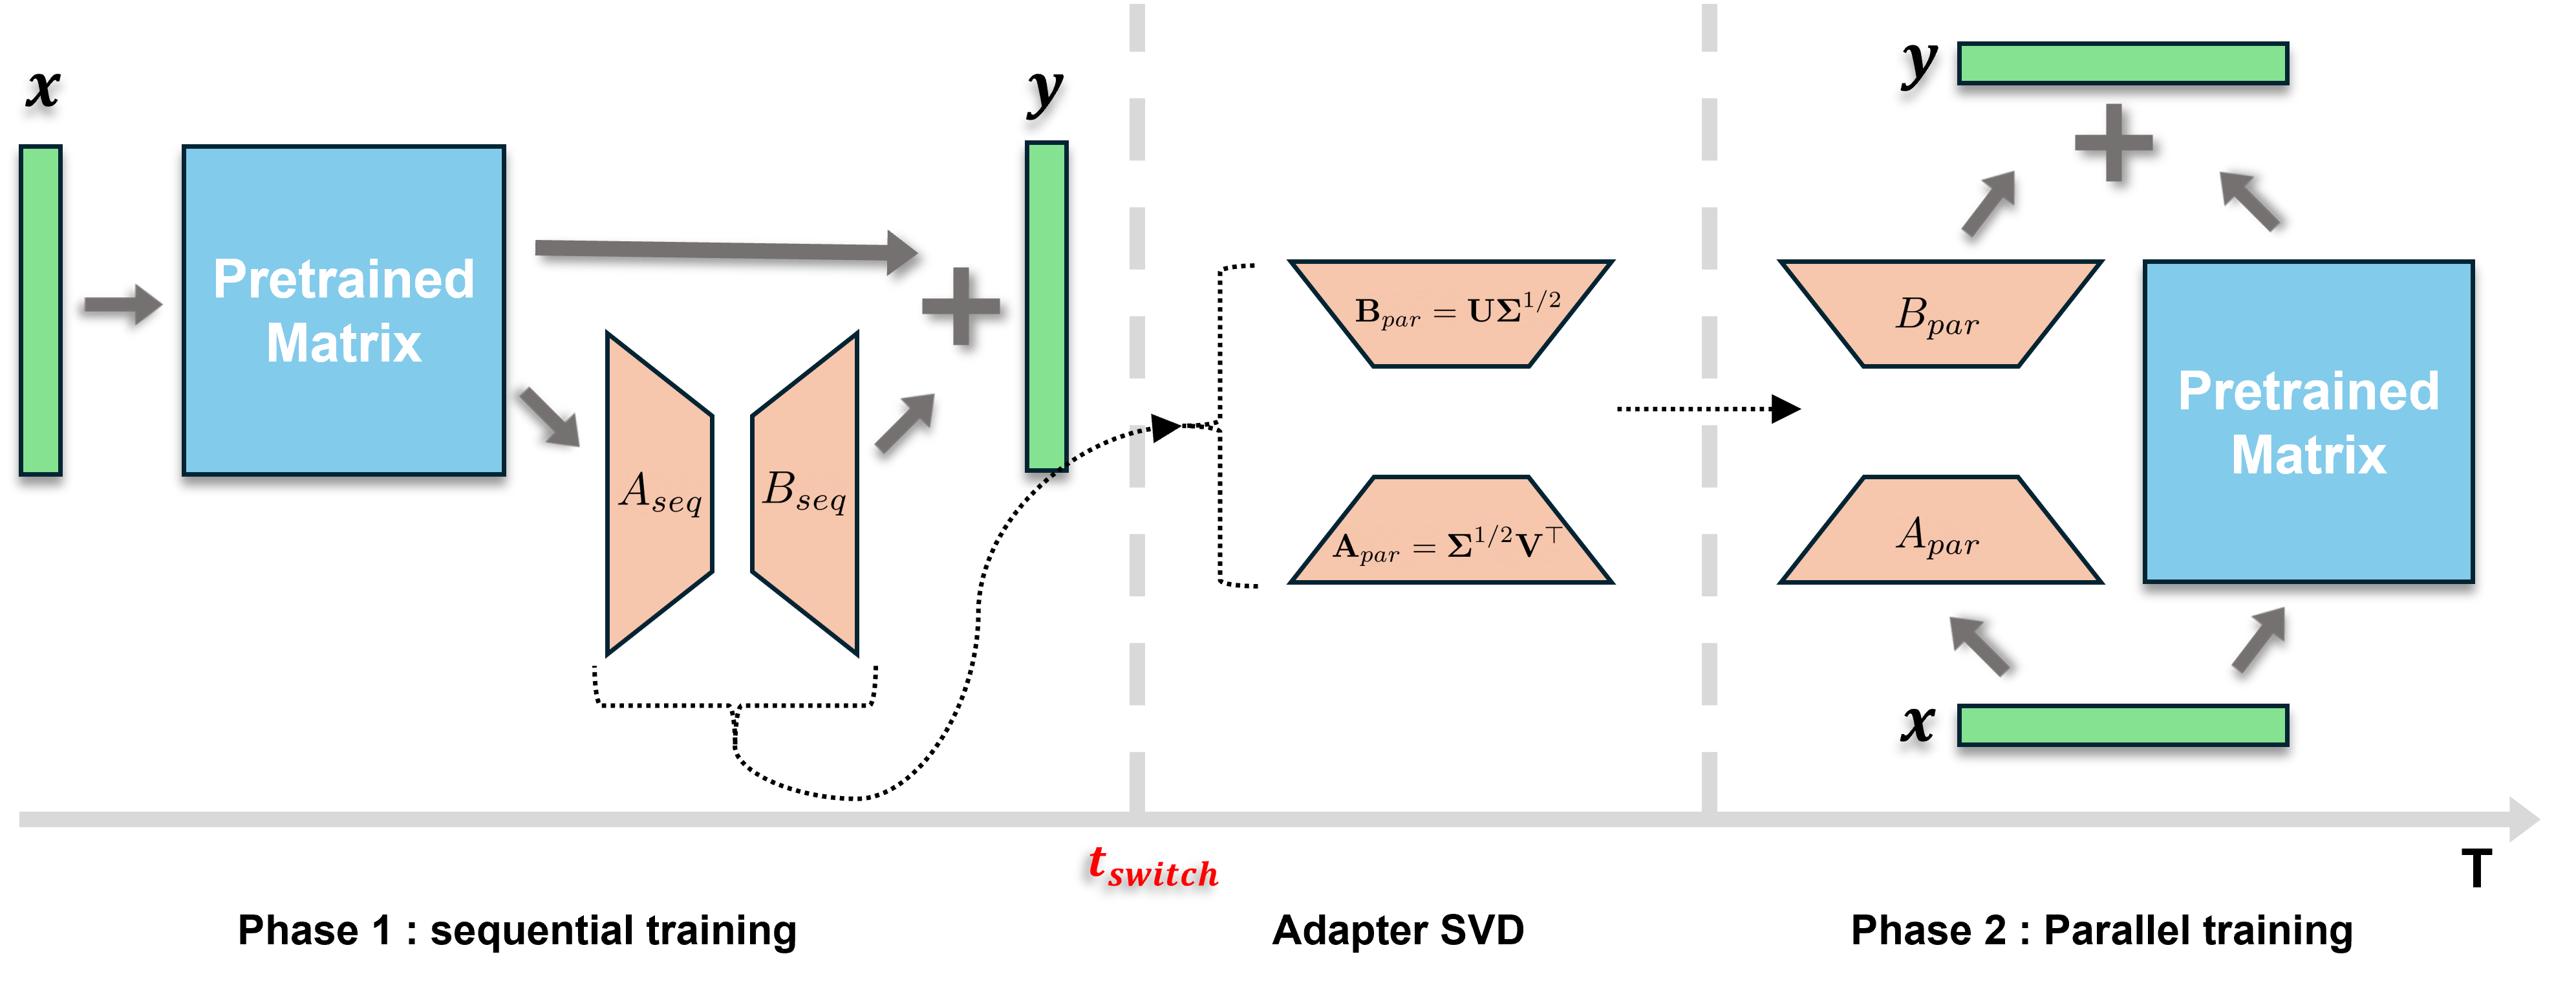
\includegraphics[width=\textwidth]{figures/fig1c.png}
    \caption{\jelly{} (Ours)}
    \label{fig:arch_portal}
\end{subfigure}
\caption{\textbf{(a)} Parallel composition (LoRA): adapters are unaligned with $\Wbase$, leading to slow early convergence.
\textbf{(b)} Sequential composition (Houlsby): probes the base manifold but adds inference latency.
\textbf{(c)} \jelly{}: unifies both topologies over the training time axis ($t \in [0, 1]$). Phase~1 ($t < \Tswitch$) probes through $\Wbase$; Phase~2 ($t \ge \Tswitch$) operates in parallel after a lossless $O(dr^2)$ Task-Isomorphic Projection, with zero added inference latency. LoRA is the special case $\Tswitch\!=\!0$.}
\label{fig:architecture}
\end{figure*}

%=============================================================================
\section{Related Work}
\label{sec:related}
%=============================================================================

\paragraph{Parallel Low-Rank Adaptation and Optimization.}
LoRA~\citep{hu2022lora} injects trainable low-rank matrices in a \emph{parallel} topology to ensure zero additional inference latency.
Subsequent work optimizes training dynamics and representational capacity:
DoRA~\citep{liu2024dora} decomposes weight updates into magnitude and direction components;
LoRA+~\citep{hayou2024loraplus} assigns distinct learning rates for $A$ and $B$ to address gradient imbalance;
AdaLoRA~\citep{zhang2023adalora} distributes rank budgets based on singular value importance; and
DyLoRA~\citep{valipour2022dylora} trains across multiple ranks simultaneously.
All of these constrain the adapter to a \emph{static} parallel topology, bypassing the pretrained manifold during early optimization.

\paragraph{The SVD Initialization Bottleneck.}
PiSSA~\citep{meng2024pissa} initializes parallel adapters using the principal singular components of $\Wbase$, accelerating convergence but requiring $O(d^3)$ full SVD per layer.
Because this decomposition occurs before observing any data, it remains \emph{task-agnostic}.
\jelly{} delays decomposition to the switching point $\Tswitch$, requiring only an $O(dr^2)$ double SVD on a learned, \emph{task-aware} matrix.

\paragraph{Sequential Topologies and Time-Axis Generalization.}
Houlsby adapters~\citep{houlsby2019parameter} use a \emph{sequential} topology, inserting bottleneck layers after pretrained layers so the adapter operates on $\Wbase x$. AdapterFusion~\citep{pfeiffer2020adapterfusion} combines multiple such adapters via attention.
Sequential adapters incur inference latency proportional to model depth, which led to their abandonment.
\jelly{} resolves this by generalizing the topology over the training time axis: a lossless \emph{Task-Isomorphic Projection} transfers the sequential adapter's manifold-aligned representations into the zero-latency parallel structure.

\paragraph{Intrinsic Dimensionality and Broad PEFT Paradigms.}
The intrinsic dimensionality perspective~\citep{aghajanyan2021intrinsic} shows that over-parameterized models can be fine-tuned within a low-dimensional subspace.
BitFit~\citep{zaken2022bitfit} optimizes only bias terms, Delta-LoRA~\citep{zi2023delta} propagates adapter deltas back to the base weights, and QLoRA~\citep{dettmers2023qlora} enables LoRA on quantized models.
\jelly{} is compatible with these paradigms; its activation-based probing and lightweight projection work directly with quantized base models.

%=============================================================================
\section{Methodology}
\label{sec:method}
%=============================================================================

\subsection{Preliminaries}

Consider a pretrained linear layer $\Wbase \in \mathbb{R}^{d_{\mathrm{out}} \times d_{\mathrm{in}}}$ and a low-rank adapter $(B \in \mathbb{R}^{d_{\mathrm{out}} \times r},\; A \in \mathbb{R}^{r \times d_{\mathrm{in}}})$ with $r \ll \min(d_{\mathrm{out}}, d_{\mathrm{in}})$.
PEFT methods differ in how the adapter receives its input.
\textbf{Parallel} adapters (LoRA) compute $h = \Wbase x + BAx$; \textbf{sequential} adapters (Houlsby) compute $h = \Wbase x + BA(\Wbase x)$.

\begin{table}[h]
\caption{PEFT adapter topologies, initialization, and gradient dynamics.}
\label{tab:topology}
\centering
\small
\resizebox{\linewidth}{!}{%
\begin{tabular}{lcccc}
\toprule
& \textbf{LoRA (Parallel)} & \textbf{Houlsby (Sequential)} & \textbf{PiSSA (Parallel)} & \textbf{\jelly{} (Ours)} \\
\midrule
Forward Pass          & $\Wbase x + BAx$           & $\Wbase x + BA(\Wbase x)$ & $\Wbase x + BAx$ & $\Wbase x + BA(\Wbase x) \to \Wbase x + BAx$ \\
Adapter Input         & $x$             & $\Wbase x$  & $x$ & $\Wbase x \to x$ \\
Effective $\Delta W$  & $BA$                   & $BA\Wbase$ & $BA$ & $BA\Wbase \to BA$ \\
$\nabla_A \mathcal{L}$ & $B^\top \delta \, x^\top$ & $B^\top \delta \, (\Wbase x)^\top$ & $B^\top \delta \, x^\top$ & $B^\top \delta \, (\Wbase x)^\top \to B^\top \delta \, x^\top$ \\
\midrule
SVD Target      & N/A & N/A & $\Wbase \in \mathbb{R}^{d \times d}$ & Core $\in \mathbb{R}^{r \times r}$ \\
Init.\ Cost    & $O(1)$         & $O(1)$ & $O(d^3)$ & $O(dr^2)$ \\
Task-Aware         & \ding{55}             & \ding{55}    & \ding{55}  & \ding{51} \\
Infer.\ Overhead     & None           & $O(dr)$/layer  & None & None \\
\bottomrule
\end{tabular}}
\end{table}

Let $\delta \triangleq \partial \mathcal{L}/\partial h$.
The key difference is in gradient structure: the sequential gradient $\nabla_A \mathcal{L} = B^\top \delta\, (\Wbase x)^\top$ biases early updates toward the principal directions of $\Wbase$, while the parallel gradient $\nabla_A \mathcal{L} = B^\top \delta\, x^\top$ treats all input directions uniformly (Table~\ref{tab:topology}).
PiSSA compensates via SVD-based initialization but at $O(d^3)$ cost per layer and without task awareness.
\jelly{} combines the gradient advantage of sequential probing with the inference efficiency of parallel adapters, using only an $O(dr^2)$ projection at the switching point.

\subsection{\jelly{}: Time-Axis Generalization}
\label{sec:portal}

Let $t \in [0, 1]$ denote the normalized training epoch. \jelly{} operates in sequential mode for $t < \Tswitch$ and parallel mode for $t \geq \Tswitch$:

\begin{equation}
h(t) = \Wbase x + B(t) A(t) \cdot
\begin{cases}
\Wbase x & \text{if } t < \Tswitch \quad (\text{Sequential Phase})\\
x & \text{if } t \geq \Tswitch \quad (\text{Parallel Phase})
\end{cases}
\label{eq:portal}
\end{equation}

Setting $\Tswitch = 0$ recovers standard LoRA; $\Tswitch = 1$ yields a pure sequential adapter.
We denote weights during the sequential phase as $\Bseq, \Aseq$ and the parallel phase as $\Bpar, \Apar$.


\subsection{Task-Isomorphic Projection via Rank-Bounded SVD}
\label{sec:projection}

At $t = \Tswitch$, we convert the sequential adapter $(\Bseq, \Aseq)$ into a parallel adapter $(\Bpar, \Apar)$ that preserves the forward output for any input $x$:
\begin{equation}
\Bpar \Apar x = \Bseq \Aseq (\Wbase x) \quad \Longrightarrow \quad \Bpar \Apar = \Bseq \Aseq \Wbase \triangleq M
\label{eq:equivalence}
\end{equation}

\paragraph{Rank bound.}
Since $M = \Bseq \Aseq \Wbase$ with $\Bseq \in \mathbb{R}^{d_{\mathrm{out}} \times r}$, the rank of $M$ is bounded:
\begin{equation*}
    \mathrm{rank}(M) \leq r
\end{equation*}

This bound enables an $O(dr^2)$ factorization instead of the $O(d^3)$ full-weight SVD:


\begin{itemize}
    \item \textbf{Step 1 (Double QR).} Extract orthogonal bases via thin QR on the sequential components:
    \begin{equation}
    \Bseq = Q_B R_B, \quad (\Aseq \Wbase)^\top = Q_X R_X
    \end{equation}
    
    \item \textbf{Step 2 (Core SVD).} Decompose the $r \times r$ core matrix $R_B R_X^\top$ and reconstruct the singular vectors of $M$:
    \begin{align}
    R_B R_X^\top &= \widetilde{U} \Sigma \widetilde{V}^\top \quad \text{(Core SVD)} \\
    M &= \underbrace{(Q_B \widetilde{U})}_{U} \Sigma \underbrace{(\widetilde{V}^\top Q_X^\top)}_{V^\top} \quad \text{(Reconstruction)}
    \end{align}
    
    \item \textbf{Step 3 (Symmetric Split).} Distribute singular values equally between the two adapters:
    \begin{equation}
    \Bpar = U \Sigma^{1/2}, \quad \Apar = \Sigma^{1/2} V^\top
    \end{equation}
\end{itemize}

\paragraph{Why symmetric splitting.}
An asymmetric factorization (e.g., $B' = U\Sigma$, $A' = V^\top$) creates a scale imbalance that destabilizes gradients after the switch. The symmetric split minimizes this:

\begin{theorem}[Optimal Conditioning]
\label{thm:condition}
Given the factorization $M = U \Sigma V^\top$, consider all rank-$r$ decompositions $M = B'A'$ where $B' = U\Sigma^\alpha$ and $A' = \Sigma^{1-\alpha} V^\top$ for $\alpha \in [0,1]$. The symmetric split ($\alpha = 1/2$) is the unique solution that minimizes the maximum condition number:
\begin{equation*}
    \min_{\alpha \in [0,1]} \max \left( \kappa(B'), \kappa(A') \right) = \sqrt{\kappa(M)}
\end{equation*}
\end{theorem}

Setting $\alpha=1/2$ equalizes the conditioning of both matrices (proof in Appendix~\ref{app:proofs}).

\paragraph{Transition stability.}
Two mechanisms ensure a smooth switch at $\Tswitch$:
\begin{itemize}
    \item \textbf{Loss invariance.} Eq.~\ref{eq:equivalence} guarantees $h(\Tswitch^-) = h(\Tswitch^+)$, so the loss passes through the boundary without discontinuity.
    \item \textbf{Momentum reset.} The optimizer's momentum and variance accumulators encode curvature from the sequential space, which is invalid after projection. We reset both to zero at $\Tswitch$~\citep{loshchilov2019adamw}.
\end{itemize}

\begin{algorithm}[t]
\caption{\jelly{}: Time-Axis Generalized Training via Task-Isomorphic Projection}
\label{alg:portal}
\begin{algorithmic}[1]
\REQUIRE Pretrained weight $\Wbase \in \mathbb{R}^{d_{out} \times d_{in}}$, rank $r$, switch step $\Tswitch$, total steps $T$
\STATE Initialize $A_{seq} \sim \mathcal{U}_{\text{Kaiming}}, \quad B_{seq} \sim \mathcal{N}(0, 10^{-4})$
\STATE Initialize optimizer states $m \gets \mathbf{0}, \quad v \gets \mathbf{0}$
\FOR{$t = 1$ \TO $T$}
    \IF{$t = \Tswitch$}
        \STATE $M \gets B_{seq} A_{seq} \Wbase$ \hfill $\triangleright$ Construct $M$
        \STATE $U, \Sigma, V^\top \gets \textsc{SVD}_r(M)$ \hfill $\triangleright$ SVD projection
        \STATE $A_{par} \gets \Sigma^{1/2} V^\top, \quad B_{par} \gets U\Sigma^{1/2}$ \hfill $\triangleright$ Energy splitting
        \STATE $m \gets \mathbf{0}, \quad v \gets \mathbf{0}$ \hfill $\triangleright$ Momentum reset
    \ENDIF
    
    \IF{$t < \Tswitch$}
        \STATE $h \gets (\mathbf{I} + B_{seq} A_{seq}) \Wbase x$ \hfill $\triangleright$ Sequential forward
    \ELSE
        \STATE $h \gets (\Wbase + B_{par} A_{par}) x$ \hfill $\triangleright$ Parallel forward
    \ENDIF
    
    \STATE $\mathcal{L} \gets \text{Loss}(h, y)$
    \STATE $(A, B), m, v \gets \text{Step}(\nabla_{\{A,B\}} \mathcal{L}, m, v)$ \hfill $\triangleright$ Update 
\ENDFOR
\STATE \textbf{return} $\Wbase + B_{par} A_{par}$ \hfill
\end{algorithmic}
\end{algorithm}

%=============================================================================
\section{Experiments}
\label{sec:experiments}
%=============================================================================

We evaluate \jelly{} on natural language understanding (NLU), generation, and reasoning benchmarks, with an emphasis on (i) end-task accuracy, (ii) sensitivity to the switching point $\Tswitch$, and (iii) efficiency at deployment.

\subsection{Experimental Setup}
\label{sec:setup}

\paragraph{Backbones and tasks.}
We evaluate two model scales.
\textbf{NLU:} DeBERTa-v3-base~\citep{he2023debertav3} on seven GLUE tasks~\citep{wang2019glue}.
\textbf{NLG:} LLaMA-2-7B~\citep{touvron2023llama2}, Mistral-7B, and Gemma-7B on mathematical reasoning (MetaMathQA~\citep{yu2024metamath} $\rightarrow$ GSM8K~\citep{cobbe2021gsm8k}, MATH~\citep{hendrycks2021math}), code generation (CodeFeedback~\citep{zhuo2024codefeedback} $\rightarrow$ HumanEval~\citep{chen2021humaneval}, MBPP~\citep{austin2021mbpp}), and conversation (WizardLM~\citep{xu2024wizardlm} $\rightarrow$ MT-Bench~\citep{zheng2023mtbench}).

\paragraph{Baselines and parameter budget.}
We compare against LoRA~\citep{hu2022lora}, PiSSA~\citep{meng2024pissa}, DoRA~\citep{liu2024dora}, AdaLoRA~\citep{zhang2023adalora}, BitFit~\citep{zaken2022bitfit}, and full fine-tuning.
Unless stated otherwise, rank is $r=8$ for DeBERTa-v3 and $r=128$ for 7B models.
For DeBERTa, adapters are inserted in attention projections $(W_q, W_k, W_v)$.
For 7B models, adapters target $(W_q, W_k, W_v, W_o)$.

\paragraph{Training protocol.}
Models are fine-tuned with matched optimizer and scheduler settings across baselines.
\jelly{} uses a validation-selected switching point $\Tswitch$ (ablation in Section~\ref{sec:ablation}).
All metrics use standard task protocols (accuracy/F1/correlation for GLUE, pass@1 for code, and MT-Bench score for conversation).

%-----------------------------------------------------------------------------
\subsection{Main Results}
\label{sec:main_results}
%-----------------------------------------------------------------------------

\paragraph{NLU.}
Table~\ref{tab:nlu} shows that \jelly{} achieves the best average score (87.24), improving over LoRA (86.52), PiSSA (86.56), and DoRA (86.58) at the same trainable-parameter scale (0.24\%).
Compared with full fine-tuning, \jelly{} is competitive while updating $>400\times$ fewer parameters.

\begin{table}[!ht]
\caption{GLUE results on DeBERTa-v3-base. Mean and standard deviation are computed over 5 seeds. Best and second-best PEFT scores are marked in \textbf{bold} and \underline{underline}.}
\label{tab:nlu}
\centering
\small
\resizebox{\linewidth}{!}{%
\begin{tabular}{llcccccccc}
\toprule
\textbf{Method} & \textbf{Params} & \textbf{SST-2} & \textbf{RTE} & \textbf{MNLI} & \textbf{MRPC} & \textbf{CoLA} & \textbf{QNLI} & \textbf{STS-B} & \textbf{Avg.} \\
\midrule
Full FT            & 184.4M (100\%) & 91.44 \scriptsize{$\pm$ 3.38} & \textbf{83.48} \scriptsize{$\pm$ 0.70} & 87.14 \scriptsize{$\pm$ 1.77} & \textbf{91.40} \scriptsize{$\pm$ 1.02} & 66.38 \scriptsize{$\pm$ 2.38} & 92.36 \scriptsize{$\pm$ 0.94} & \textbf{91.10} \scriptsize{$\pm$ 0.07} & 86.18 \\
LoRA              & 0.44M (0.24\%) & 95.52 \scriptsize{$\pm$ 0.23} & 81.14 \scriptsize{$\pm$ 1.66} & 90.04 \scriptsize{$\pm$ 0.15} & 89.02 \scriptsize{$\pm$ 0.91} & 66.68 \scriptsize{$\pm$ 1.53} & 93.68 \scriptsize{$\pm$ 0.18} & 89.66 \scriptsize{$\pm$ 0.44} & 86.52 \\
LoRA (Gauss.)     & 0.44M (0.24\%) & 95.64 \scriptsize{$\pm$ 0.21} & 80.42 \scriptsize{$\pm$ 2.21} & 90.00 \scriptsize{$\pm$ 0.16} & 89.64 \scriptsize{$\pm$ 0.42} & \underline{67.50} \scriptsize{$\pm$ 1.09} & 93.68 \scriptsize{$\pm$ 0.18} & 89.96 \scriptsize{$\pm$ 0.67} & \underline{86.70} \\
PiSSA             & 0.44M (0.24\%) & \underline{95.70} \scriptsize{$\pm$ 0.29} & 79.92 \scriptsize{$\pm$ 2.65} & \underline{90.12} \scriptsize{$\pm$ 0.11} & 89.64 \scriptsize{$\pm$ 0.87} & 66.20 \scriptsize{$\pm$ 0.95} & \textbf{93.98} \scriptsize{$\pm$ 0.19} & 90.46 \scriptsize{$\pm$ 0.29} & 86.56 \\
DoRA              & 0.47M (0.25\%) & 95.44 \scriptsize{$\pm$ 0.21} & 81.36 \scriptsize{$\pm$ 1.99} & 90.00 \scriptsize{$\pm$ 0.10} & 88.92 \scriptsize{$\pm$ 0.76} & 66.94 \scriptsize{$\pm$ 1.51} & 93.66 \scriptsize{$\pm$ 0.21} & 89.72 \scriptsize{$\pm$ 0.48} & 86.58 \\
AdaLoRA           & 0.44M (0.24\%) & 94.28 \scriptsize{$\pm$ 0.23} & 56.88 \scriptsize{$\pm$ 2.46} & 89.70 \scriptsize{$\pm$ 0.07} & 74.80 \scriptsize{$\pm$ 0.00} & 55.12 \scriptsize{$\pm$ 0.69} & 92.42 \scriptsize{$\pm$ 0.16} & 87.34 \scriptsize{$\pm$ 0.13} & 78.64 \\
BitFit            & 0.10M (0.05\%) & 95.06 \scriptsize{$\pm$ 0.23} & 76.92 \scriptsize{$\pm$ 0.65} & 89.72 \scriptsize{$\pm$ 0.08} & 87.98 \scriptsize{$\pm$ 0.36} & 64.36 \scriptsize{$\pm$ 1.09} & 93.08 \scriptsize{$\pm$ 0.08} & \underline{90.52} \scriptsize{$\pm$ 0.13} & 85.38 \\
\midrule
\textbf{\jelly{}} & 0.44M (0.24\%) & \textbf{95.98} \scriptsize{$\pm$ 0.16} & \underline{82.60} \scriptsize{$\pm$ 2.11} & \textbf{90.30} \scriptsize{$\pm$ 0.10} & \underline{90.22} \scriptsize{$\pm$ 1.42} & \textbf{67.86} \scriptsize{$\pm$ 0.84} & \underline{93.94} \scriptsize{$\pm$ 0.13} & 90.00 \scriptsize{$\pm$ 0.35} & \textbf{87.24} \\
\bottomrule
\end{tabular}}
\end{table}

\paragraph{NLG.}
Table~\ref{tab:nlg_comprehensive} reports results across three 7B backbones.
\jelly{} is strongest on Mistral-7B and Gemma-7B in aggregate, with clear gains on MATH/MBPP/HumanEval in most settings.
On LLaMA-2-7B, \jelly{} improves reasoning and coding metrics while LoRA remains slightly stronger on MT-Bench.

\begin{table}[!ht]
\caption{NLG results on 7B backbones. \jelly{} reports the best switching configuration from the corresponding sweep for each backbone/task family. Best and second-best scores per backbone are marked in \textbf{bold} and \underline{underline}.}
\label{tab:nlg_comprehensive}
\centering
\small
\resizebox{\linewidth}{!}{%
\begin{tabular}{ll ccccc | c}
\toprule
& & \multicolumn{2}{c}{\textbf{Math}} & \multicolumn{2}{c}{\textbf{Code}} & \textbf{Conv.} & \\
\cmidrule(lr){3-4} \cmidrule(lr){5-6} \cmidrule(lr){7-7}
\textbf{Model} & \textbf{Method} & \textbf{GSM8K$\uparrow$} & \textbf{MATH$\uparrow$} & \textbf{HumanEval$\uparrow$} & \textbf{MBPP$\uparrow$} & \textbf{MT-Bench$\uparrow$} & \textbf{Avg.} \\
\midrule
\multirow{3}{*}{LLaMA-2-7B}
& Sequential      & 54.67 \scriptsize{$\pm$ 1.29} & \underline{9.13} \scriptsize{$\pm$ 0.23} & 29.90 \scriptsize{$\pm$ 0.60} & 42.10 \scriptsize{$\pm$ 1.39} & 6.12 \scriptsize{$\pm$ 0.03} & 28.38 \\
& LoRA            & \underline{55.10} \scriptsize{$\pm$ 1.60} & 8.70 \scriptsize{$\pm$ 0.26} & \underline{30.87} \scriptsize{$\pm$ 2.76} & \underline{44.00} \scriptsize{$\pm$ 0.95} & \textbf{6.29} \scriptsize{$\pm$ 0.04} & \underline{28.99} \\
& \textbf{\jelly{} (Ours)} & \textbf{56.90} & \textbf{9.30} & \textbf{31.70} & \textbf{43.40} & \underline{6.12} & \textbf{29.48} \\
\midrule
\multirow{3}{*}{Mistral-7B}
& Sequential      & \underline{69.10} \scriptsize{$\pm$ 0.52} & \underline{17.47} \scriptsize{$\pm$ 0.85} & \underline{48.75} \scriptsize{$\pm$ 3.46} & \textbf{60.60} \scriptsize{$\pm$ 0.71} & \textbf{6.95} \scriptsize{$\pm$ 0.08} & \underline{40.57} \\
& LoRA            & 68.17 \scriptsize{$\pm$ 0.91} & 16.87 \scriptsize{$\pm$ 0.57} & 46.35 \scriptsize{$\pm$ 1.77} & 57.80 \scriptsize{$\pm$ 2.40} & 6.75 \scriptsize{$\pm$ 0.01} & 39.19 \\
& \textbf{\jelly{} (Ours)} & \textbf{70.00} \scriptsize{$\pm$ 0.50} & \textbf{18.00} & \textbf{50.00} & \textbf{60.60} & \underline{6.94} & \textbf{41.11} \\
\midrule
\multirow{3}{*}{Gemma-7B}
& Sequential      & 71.27 \scriptsize{$\pm$ 0.67} & 21.23 \scriptsize{$\pm$ 0.58} & \underline{51.20} \scriptsize{$\pm$ 1.70} & \underline{60.70} \scriptsize{$\pm$ 0.57} & 6.81 & \underline{42.24} \\
& LoRA            & \textbf{71.50} \scriptsize{$\pm$ 0.26} & \textbf{21.90} \scriptsize{$\pm$ 0.10} & 50.30 \scriptsize{$\pm$ 2.12} & 60.45 \scriptsize{$\pm$ 2.05} & \underline{6.91} & 42.21 \\
& \textbf{\jelly{} (Ours)} & \underline{70.50} & \underline{21.20} & \textbf{55.50} \scriptsize{$\pm$ 0.85} & \textbf{62.70} & \textbf{7.03} & \textbf{43.39} \\
\bottomrule
\end{tabular}}
\end{table}

\paragraph{Sarcasm detection.}
Table~\ref{tab:sarcasm} shows that \jelly{} achieves the strongest PEFT average score (81.56), with the best Headlines and Sarc performance.
Full fine-tuning remains best on iSarcasm, which is consistent with its low-data regime.

\begin{table}[!ht]
\caption{Sarcasm detection on DeBERTa-v3-base. Mean and standard deviation are computed over 5 seeds. Best and second-best PEFT scores are marked in \textbf{bold} and \underline{underline}.}
\label{tab:sarcasm}
\centering
\footnotesize
\renewcommand{\arraystretch}{1.2}
\setlength{\tabcolsep}{7pt}
\begin{tabular}{llcccc}
\toprule
\textbf{Method} & \textbf{Params} & \textbf{Headlines} & \textbf{iSarcasm} & \textbf{Sarc} & \textbf{Avg.} \\
\midrule
Full FT            & 184.4M (100\%) & \underline{94.20} & \textbf{79.50} & \textbf{73.10} & \textbf{82.27} \\
LoRA              & 0.44M (0.24\%) & 93.15 \scriptsize{$\pm$ 0.48} & 78.04 \scriptsize{$\pm$ 0.51} & 72.09 \scriptsize{$\pm$ 0.22} & 81.09 \\
PiSSA             & 0.44M (0.24\%) & 92.83 \scriptsize{$\pm$ 0.65} & 77.41 \scriptsize{$\pm$ 0.94} & 72.29 \scriptsize{$\pm$ 0.23} & 80.84 \\
DoRA              & 0.47M (0.25\%) & 93.19 \scriptsize{$\pm$ 0.47} & 77.81 \scriptsize{$\pm$ 0.53} & 71.98 \scriptsize{$\pm$ 0.21} & 81.02 \\
AdaLoRA           & 0.44M (0.24\%) & 87.94 \scriptsize{$\pm$ 0.35} & 74.93 \scriptsize{$\pm$ 0.00} & 65.51 \scriptsize{$\pm$ 0.86} & 76.13 \\
\midrule
\rowcolor[gray]{.95}\textbf{\jelly{}} & 0.44M (0.24\%) & \textbf{93.50} \scriptsize{$\pm$ 0.43} & \underline{78.63} \scriptsize{$\pm$ 0.70} & \underline{72.55} \scriptsize{$\pm$ 0.16} & \underline{81.56} \\
\bottomrule
\end{tabular}
\end{table}

%-----------------------------------------------------------------------------
\subsection{Switching Point Ablation}
\label{sec:ablation}
%-----------------------------------------------------------------------------

We study how performance changes with $\Tswitch$.
For NLU and sarcasm we sweep $\{10\%, 30\%, 50\%\}$; for NLG we sweep $\{20\%, 50\%, 80\%\}$.
The ablations support a key trend: different tasks prefer different sequential probing lengths.

\begin{table}[!ht]
\caption{$\Tswitch$ ablation on GLUE (DeBERTa-v3-base, $r=8$, 5-seed mean). $\Tswitch=0\%$ corresponds to LoRA.}
\label{tab:nlu_ablation}
\centering
\footnotesize
\setlength{\tabcolsep}{4pt}
\begin{tabular}{l | ccccccc | c}
\toprule
$\Tswitch$ & \textbf{CoLA} & \textbf{MNLI} & \textbf{MRPC} & \textbf{QNLI} & \textbf{RTE} & \textbf{SST-2} & \textbf{STS-B} & \textbf{Avg.} \\
\midrule
0\% (LoRA) & 66.74 & 90.04 & 89.02 & 93.68 & 81.14 & 95.52 & 89.66 & 86.54 \\
10\%       & \textbf{67.86} & 90.24 & 89.06 & \textbf{93.94} & 79.14 & 95.66 & 88.98 & 86.41 \\
30\%       & 67.64 & \textbf{90.30} & 89.96 & 93.92 & 81.20 & 95.88 & 89.74 & 86.95 \\
50\%       & 67.58 & 90.26 & \textbf{90.22} & 93.92 & \textbf{82.62} & \textbf{95.98} & \textbf{90.04} & \textbf{87.23} \\
\bottomrule
\end{tabular}
\end{table}

\begin{table}[!ht]
\caption{$\Tswitch$ ablation on NLG backbones ($r=128$, seed 42).}
\label{tab:nlg_ablation}
\centering
\footnotesize
\renewcommand{\arraystretch}{1.1}
\setlength{\tabcolsep}{6pt}
\begin{tabular}{ll | ccc | c}
\toprule
\textbf{Backbone} & $\Tswitch$ & \textbf{GSM8K} & \textbf{MBPP} & \textbf{MATH} & \textbf{Avg.} \\
\midrule
\multirow{4}{*}{LLaMA-2-7B}
    & 0\% (LoRA) & 56.70 & 43.10 & 8.80 & 36.20 \\
    & 20\%       & \textbf{56.90} & 41.80 & 9.30 & 36.00 \\
    & 50\%       & 55.60 & 40.50 & 9.00 & 35.03 \\
    & 80\%       & 56.60 & \textbf{43.40} & \textbf{9.50} & \textbf{36.50} \\
\midrule
\multirow{4}{*}{Mistral-7B}
    & 0\% (LoRA) & 67.50 & 56.10 & 16.70 & 46.77 \\
    & 20\%       & 68.80 & 60.10 & 18.00 & 48.97 \\
    & 50\%       & 68.00 & 58.70 & 17.50 & 48.07 \\
    & 80\%       & \textbf{69.40} & \textbf{60.60} & \textbf{18.24} & \textbf{49.41} \\
\midrule
\multirow{4}{*}{Gemma-7B}
    & 0\% (LoRA) & \textbf{71.30} & 61.90 & \textbf{22.00} & \textbf{51.73} \\
    & 20\%       & 70.50 & 61.40 & 21.00 & 50.97 \\
    & 50\%       & 70.20 & 55.80 & 21.20 & 49.07 \\
    & 80\%       & 69.50 & \textbf{62.70} & 20.80 & 51.00 \\
\bottomrule
\end{tabular}
\end{table}

\begin{table}[!ht]
\caption{$\Tswitch$ ablation on sarcasm benchmarks (DeBERTa-v3-base, $r=8$, 5-seed mean).}
\label{tab:sarc_ablation}
\centering
\footnotesize
\setlength{\tabcolsep}{9pt}
\begin{tabular}{l | ccc | c}
\toprule
$\Tswitch$ & \textbf{Headlines} & \textbf{iSarcasm} & \textbf{Sarc} & \textbf{Avg.} \\
\midrule
0\% (LoRA) & 93.15 & \textbf{78.04} & 72.09 & 81.09 \\
10\%       & \textbf{93.32} & 76.89 & \textbf{72.49} & 80.90 \\
30\%       & 93.00 & 76.95 & 72.47 & 80.81 \\
50\%       & 93.09 & \textbf{78.04} & 72.47 & \textbf{81.20} \\
\bottomrule
\end{tabular}
\end{table}

%-----------------------------------------------------------------------------
\subsection{Task and Backbone Analysis}
\label{sec:task_analysis}
%-----------------------------------------------------------------------------

The ablations show that the best $\Tswitch$ is task-dependent.
To quantify this behavior, we use two diagnostics.

\noindent\textbf{Early Gain Ratio (EGR).}
\begin{equation}
\mathrm{EGR}
=
\frac{\mathrm{score}_{10\%}-\mathrm{score}_{\mathrm{LoRA}}}
{\mathrm{score}_{\mathrm{best}}-\mathrm{score}_{\mathrm{LoRA}}}.
\label{eq:egr}
\end{equation}
Higher EGR indicates that sequential benefits are realized early, favoring smaller $\Tswitch$.

\noindent\textbf{Gain decomposition (SB--SG).}
At the best switching point $\Tswitch^\star$,
\begin{equation}
\Delta_{\text{\textsc{Jelly}}}(\Tswitch^\star)
=
\underbrace{(\mathrm{Seq}-\mathrm{LoRA})}_{\mathrm{SB}}
+
\underbrace{\left[\Delta_{\text{\textsc{Jelly}}}(\Tswitch^\star)-(\mathrm{Seq}-\mathrm{LoRA})\right]}_{\mathrm{SG}}.
\label{eq:sbsg}
\end{equation}
Here SB is the pure sequential contribution, while SG measures the additional gain from switching.

\begin{figure}[!ht]
\centering
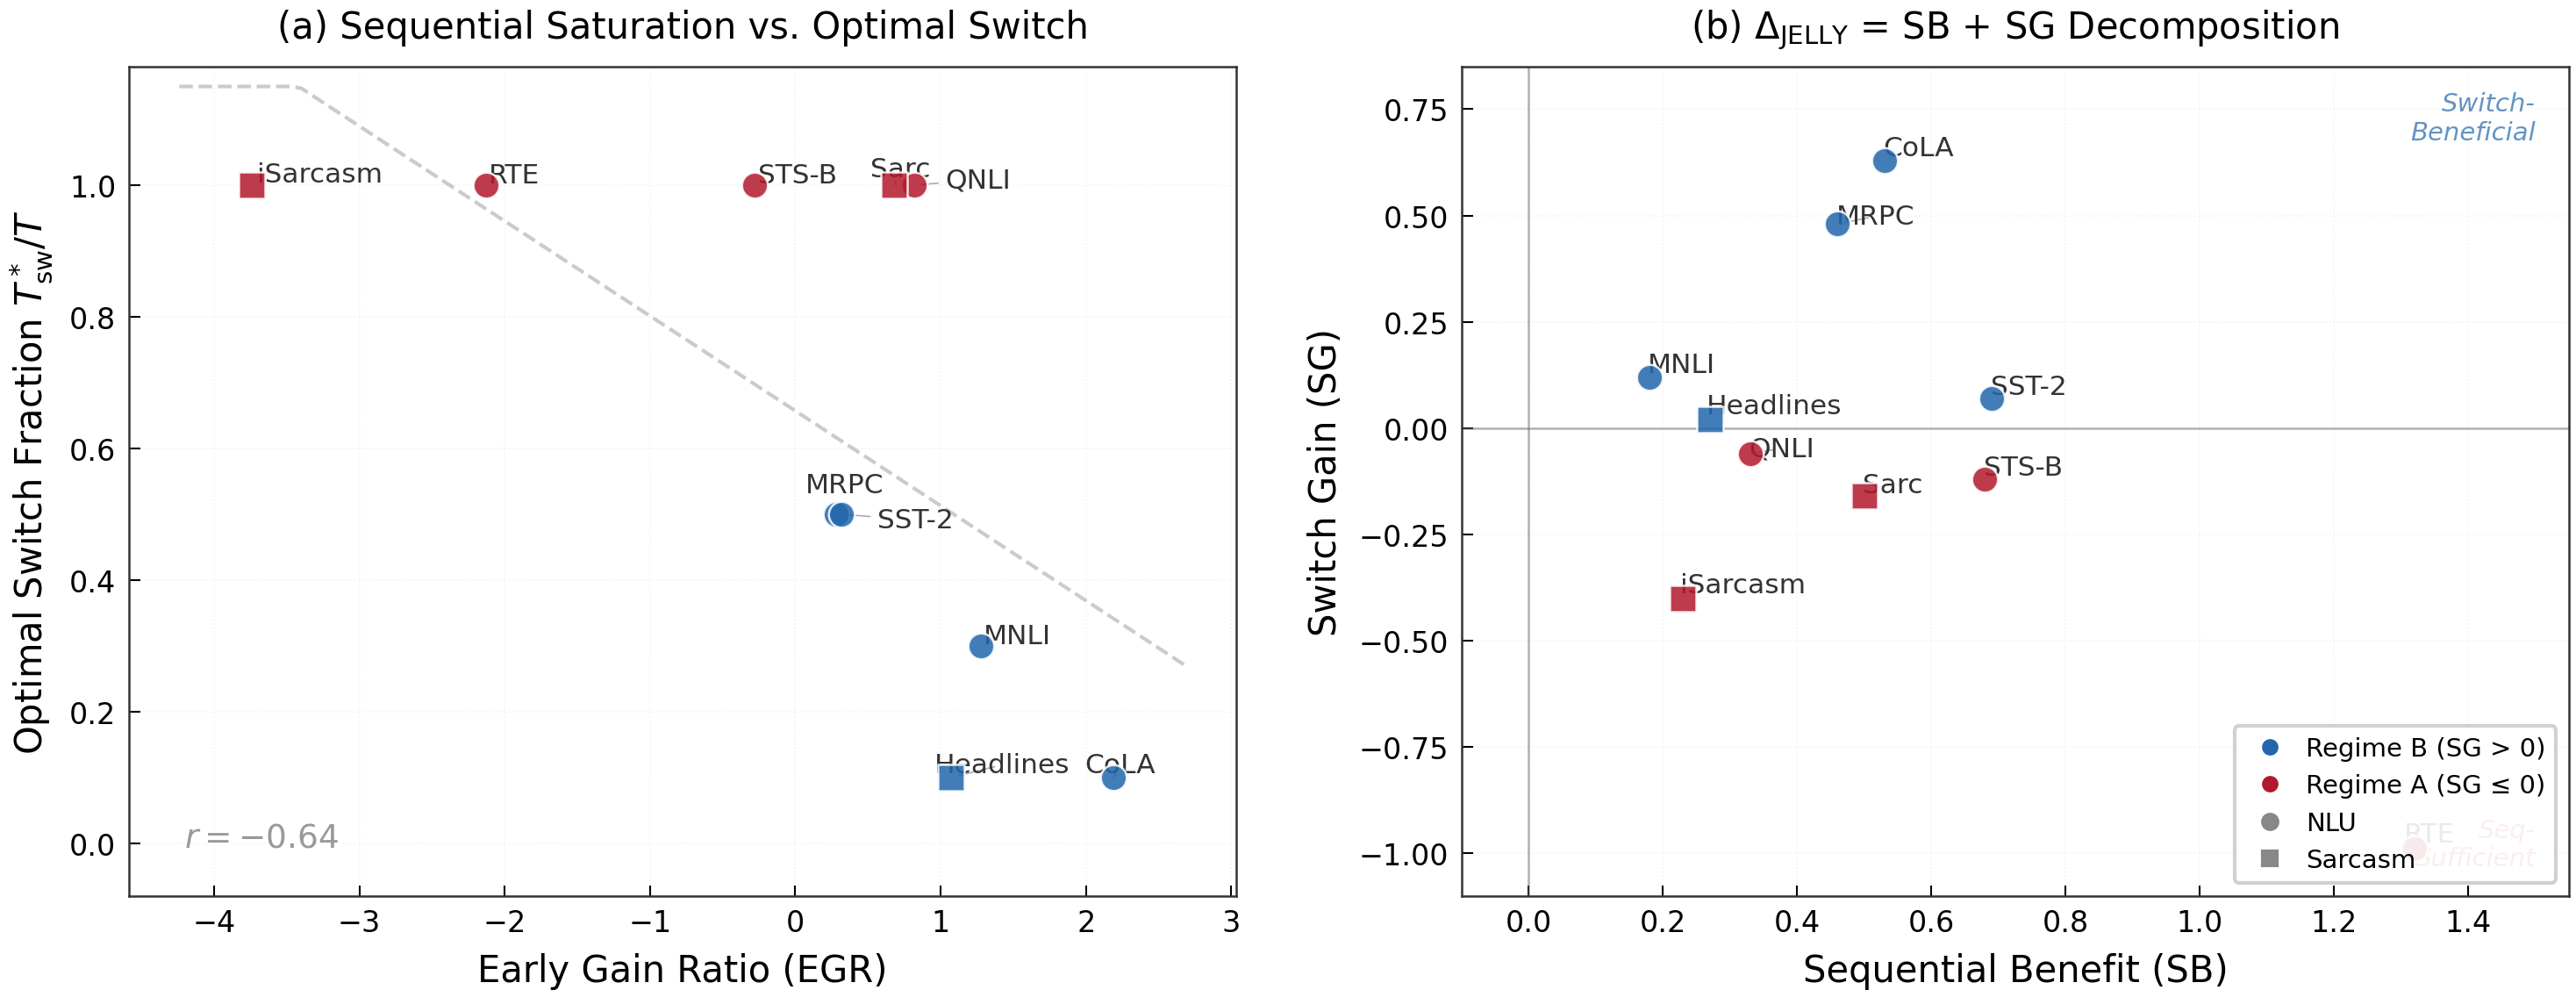
\includegraphics[width=\textwidth]{figures/figA_task_analysis.png}
\caption{\textbf{Task-level switching behavior.}
\textbf{(a)} EGR versus optimal switch fraction.
\textbf{(b)} SB--SG decomposition showing regimes where switching adds extra value ($\mathrm{SG}>0$) versus regimes dominated by sequential benefit.}
\label{fig:task_analysis}
\end{figure}

\begin{figure}[!ht]
\centering
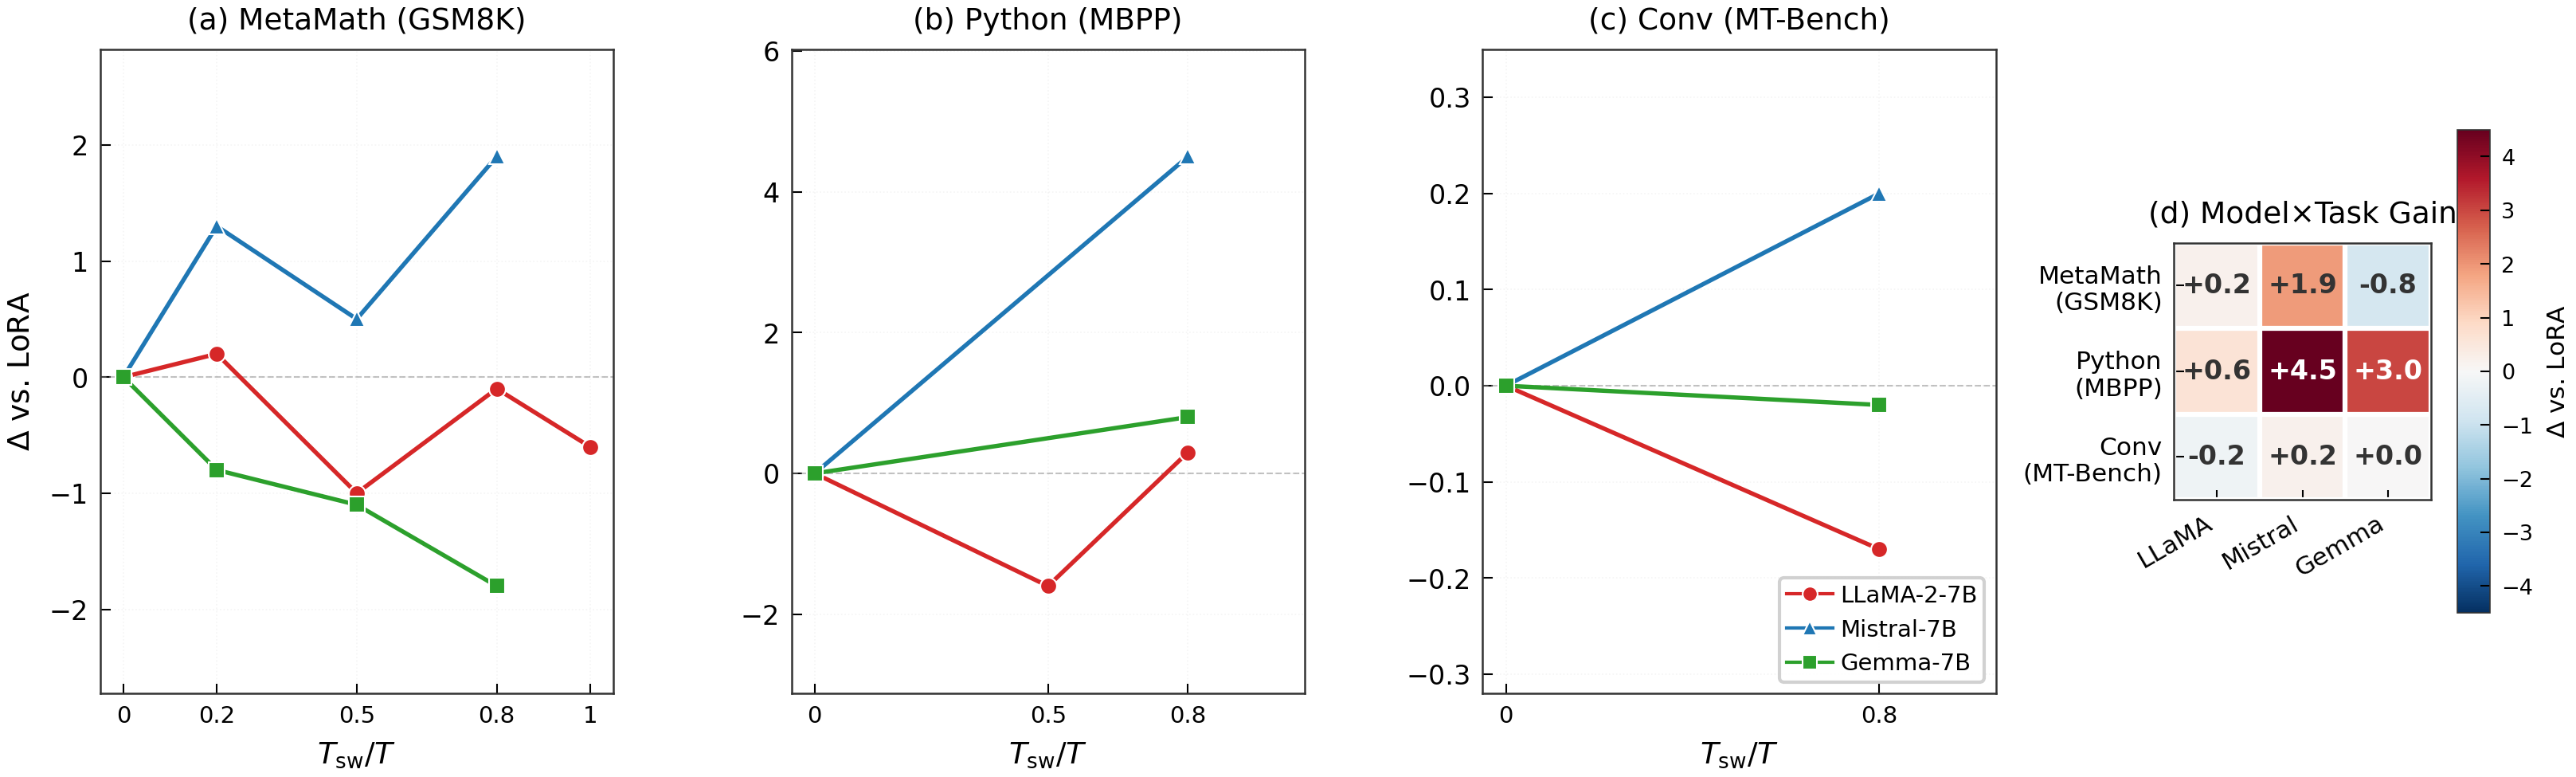
\includegraphics[width=\textwidth]{figures/figB_model_analysis.png}
\caption{\textbf{Backbone-level switching behavior.}
Performance gain versus $\Tswitch$ for LLaMA-2-7B, Mistral-7B, and Gemma-7B across task families.}
\label{fig:model_analysis}
\end{figure}

%-----------------------------------------------------------------------------
\subsection{Design Choice: Sequential $\rightarrow$ Parallel}
\label{sec:design_choice}
%-----------------------------------------------------------------------------

Why do we switch from sequential to parallel, instead of the reverse?
The answer is the optimization--deployment tradeoff.
Sequential adapters provide task-aware probing through $\Wbase x$ during early training, while parallel adapters permit weight merging and zero extra inference latency.
Reversing the order gives up early manifold-guided updates and still ends with sequential inference overhead.

\begin{table}[!ht]
\caption{Topology comparison from optimization and deployment perspectives.}
\label{tab:topology_comparison}
\centering
\footnotesize
\setlength{\tabcolsep}{8pt}
\begin{tabular}{lccc}
\toprule
\textbf{Feature} & \textbf{LoRA (Parallel)} & \textbf{Houlsby (Sequential)} & \textbf{\jelly{} (Ours)} \\
\midrule
Task-aware probing via $\Wbase x$ & \ding{55} & \ding{51} & \ding{51} \\
Inference overhead                & None & $O(dr)$/layer & None \\
Post-training weight merge        & \ding{51} & \ding{55} & \ding{51} \\
Training profile                  & Static & Static & Dynamic over $t$ \\
\bottomrule
\end{tabular}
\end{table}

%-----------------------------------------------------------------------------
\subsection{Complexity and Inference Latency}
\label{sec:complexity}
%-----------------------------------------------------------------------------

At switching time, PiSSA requires full SVD on $\Wbase\in\mathbb{R}^{d\times d}$, while \jelly{} decomposes a rank-bounded core matrix.
This yields lower initialization-time complexity without changing inference cost after merging.

\begin{table}[!ht]
\caption{Asymptotic complexity at initialization/switching time (per adapted layer).}
\label{tab:svd_complexity}
\centering
\small
\begin{tabular}{lcc}
\toprule
\textbf{Method} & \textbf{Decomposition target} & \textbf{Complexity} \\
\midrule
PiSSA & $\Wbase\in\mathbb{R}^{d\times d}$ & $O(d^3)$ \\
\jelly{} (TIP) & rank-$r$ core matrix & $O(dr^2 + r^3)$ \\
\bottomrule
\end{tabular}
\end{table}

\begin{table}[!ht]
\caption{Inference latency after training. \jelly{} and PiSSA are merge-equivalent to LoRA at inference.}
\label{tab:inference_latency}
\centering
\small
\begin{tabular}{lcc}
\toprule
\textbf{Method} & \textbf{Inference mode} & \textbf{Relative latency} \\
\midrule
LoRA                       & Parallel (merged) & $1.00\times$ \\
\jelly{} ($\Tswitch=0.2$) & Parallel (merged) & $1.00\times$ \\
\jelly{} ($\Tswitch=0.5$) & Parallel (merged) & $1.00\times$ \\
\jelly{} ($\Tswitch=0.8$) & Parallel (merged) & $1.00\times$ \\
PiSSA                      & Parallel (merged) & $1.00\times$ \\
Sequential                 & Sequential        & $> 1.00\times$ \\
\bottomrule
\end{tabular}
\end{table}

%=============================================================================
\section{Conclusion}
\label{sec:conclusion}
%=============================================================================

We presented \jelly{}, a PEFT framework that treats adapter topology as a function of training time.
The method first performs manifold-aware sequential probing, then switches to a mergeable parallel form through a lossless Task-Isomorphic Projection.
Across NLU, sarcasm, and NLG benchmarks, \jelly{} is consistently competitive with or better than strong PEFT baselines at the same parameter budget.
The switching-point analysis further suggests that $\Tswitch$ acts as a practical indicator of task--manifold alignment.

\paragraph{Limitations.}
Selecting $\Tswitch$ currently requires validation sweeps.
An adaptive switching rule based on online training signals is a natural next step.
Our largest experiments are at 7B scale; extending to larger models remains future work.

%=============================================================================
\bibliographystyle{plainnat}
\bibliography{references}

%=============================================================================
\appendix
%=============================================================================

\section{Proofs}
\label{app:proofs}

\subsection{Proof of Theorem~\ref{thm:condition}}
\begin{proof}
Let $M = U\Sigma V^\top$ with $\Sigma = \diag(\sigma_1, \ldots, \sigma_r)$ and $\sigma_1 \ge \cdots \ge \sigma_r > 0$.
For $B' = U\Sigma^\alpha$ and $A' = \Sigma^{1-\alpha}V^\top$ with $\alpha \in [0,1]$, orthogonality of $U,V$ gives
\[
\kappa(B') = \kappa(\Sigma^\alpha) = \kappa(M)^\alpha,\quad
\kappa(A') = \kappa(\Sigma^{1-\alpha}) = \kappa(M)^{1-\alpha}.
\]
Therefore,
\[
\min_{\alpha\in[0,1]} \max\{\kappa(B'),\kappa(A')\}
=
\min_{\alpha\in[0,1]} \kappa(M)^{\max(\alpha,1-\alpha)},
\]
which is uniquely minimized at $\alpha=\tfrac{1}{2}$, yielding
\[
\kappa(B')=\kappa(A')=\sqrt{\kappa(M)}.
\]
\end{proof}

\subsection{Gradient-Flow Intuition}
Let $\Wbase = U_W\Sigma_WV_W^\top$.
In sequential mode, $\nabla_A\mathcal{L}\propto(\Wbase x)^\top = x^\top V_W\Sigma_WU_W^\top$, so updates are biased toward dominant singular directions of $\Wbase$.
In parallel mode, $\nabla_A\mathcal{L}\propto x^\top$ and this spectral bias is absent.
This motivates the sequential warm-up before switching.

\section{Additional Experimental Details}
\label{app:additional}

\subsection{Per-Task Hyperparameters}
\label{app:hyperparams}

\begin{table}[!ht]
\caption{Experimental settings and selected switch fractions used in this work.}
\label{tab:master_experimental_settings_v2}
\centering
\scriptsize
\begin{tabular}{lllcccc}
\toprule
\textbf{Category} & \textbf{Backbone} & \textbf{Task} & \textbf{Epochs} & \textbf{$lr$} & \textbf{Batch} & \textbf{Switch (\%)} \\
\midrule
\multirow{7}{*}{\textbf{NLU}}
& \multirow{7}{*}{DeBERTa-v3}
& CoLA      & 10 & 5e-5 & 32 & 10 \\
& & MNLI      & 5  & 3e-5 & 32 & 10 \\
& & MRPC      & 10 & 5e-5 & 32 & 10 \\
& & QNLI      & 10 & 5e-5 & 32 & 10 \\
& & RTE       & 20 & 5e-5 & 32 & 10 \\
& & SST-2     & 10 & 5e-5 & 32 & 10 \\
& & STS-B     & 10 & 5e-5 & 32 & 10 \\
\midrule
\multirow{15}{*}{\textbf{NLG}}
& \multirow{5}{*}{LLaMA-2-7B}
& MBPP      & 3 & 2e-4 & 128 & 30 \\
& & MATH      & 5 & 2e-4 & 128 & 30 \\
& & GSM8K     & 3 & 2e-4 & 128 & 30 \\
& & HumanEval & 3 & 2e-4 & 128 & 30 \\
& & MT-Bench  & 3 & 2e-4 & 128 & 30 \\
\cmidrule{2-7}
& \multirow{5}{*}{Mistral-7B}
& MBPP      & 3 & 1e-4 & 128 & 20 \\
& & MATH      & 3 & 1e-4 & 128 & 30 \\
& & GSM8K     & 3 & 1e-4 & 128 & 20 \\
& & HumanEval & 3 & 1e-4 & 128 & 20 \\
& & MT-Bench  & 3 & 1e-4 & 128 & 30 \\
\cmidrule{2-7}
& \multirow{5}{*}{Gemma-7B}
& MBPP      & 3 & 1e-4 & 128 & 30 \\
& & MATH      & 5 & 2e-4 & 128 & 50 \\
& & GSM8K     & 3 & 1e-4 & 128 & 30 \\
& & HumanEval & 3 & 1e-4 & 128 & 30 \\
& & MT-Bench  & 5 & 2e-4 & 128 & 50 \\
\midrule
\multirow{3}{*}{\textbf{Sarcasm}}
& \multirow{3}{*}{DeBERTa-v3}
& Headlines & 10 & 1e-4 & 32 & 10 \\
& & iSarcasm  & 15 & 1e-4 & 32 & 50 \\
& & Sarc      & 3  & 1e-4 & 32 & 10 \\
\bottomrule
\end{tabular}
\end{table}

\subsection{Asynchronous Per-Module Switching}
\label{app:async}

\begin{table}[!ht]
\caption{Per-module asynchronous switching on DeBERTa-v3-base ($r=8$, 3-seed mean). $0\%$ means parallel from the start for that module.}
\label{tab:t3_async_final}
\centering
\small
\begin{tabular}{ccc|cccccc}
\toprule
\multicolumn{3}{c|}{\textbf{Switching point}} & \multicolumn{6}{c}{\textbf{GLUE tasks}} \\
$q$ & $k$ & $v$ & \textbf{SST-2} & \textbf{CoLA} & \textbf{MRPC} & \textbf{RTE} & \textbf{STS-B} & \textbf{Avg.} \\
\midrule
0\%  & 0\%  & 0\%  & 95.4 & 66.4 & 88.9 & 82.1 & 89.6 & 84.5 \\
30\% & 30\% & 30\% & 95.9 & 67.6 & 90.0 & 82.1 & 89.5 & 85.0 \\
50\% & 50\% & 50\% & 96.0 & 67.6 & 89.9 & 82.7 & 89.8 & 85.2 \\
\midrule
50\% & 0\%  & 0\%  & 95.7 & 67.2 & 88.9 & 81.8 & 89.7 & 84.7 \\
0\%  & 50\% & 0\%  & 95.5 & 67.8 & 89.6 & 81.5 & 88.8 & 84.6 \\
0\%  & 0\%  & 50\% & 95.7 & 67.1 & 89.3 & 82.8 & 88.6 & 84.7 \\
30\% & 50\% & 50\% & \textbf{96.1} & 67.7 & \textbf{90.0} & \textbf{83.0} & 89.7 & \textbf{85.3} \\
50\% & 30\% & 50\% & 95.9 & 67.2 & 89.9 & 82.3 & 89.8 & 85.0 \\
50\% & 50\% & 30\% & 96.0 & 67.5 & \textbf{90.0} & 82.2 & 89.7 & 85.1 \\
\midrule
0\%  & 30\% & 30\% & 95.9 & 67.3 & 89.7 & 81.5 & 89.7 & 84.8 \\
30\% & 0\%  & 30\% & 95.8 & 66.7 & 89.3 & 81.9 & 89.6 & 84.7 \\
30\% & 30\% & 0\%  & 95.6 & 67.4 & 89.4 & 81.9 & 89.1 & 84.7 \\
\midrule
0\%  & 30\% & 50\% & 95.8 & \textbf{67.8} & 89.7 & 81.9 & \textbf{89.8} & 85.0 \\
50\% & 30\% & 0\%  & 95.6 & 67.6 & 89.4 & 81.5 & 89.2 & 84.7 \\
\bottomrule
\end{tabular}
\end{table}

\subsection{Training Dynamics}
\label{app:training_dynamics}

\begin{figure}[!ht]
\centering
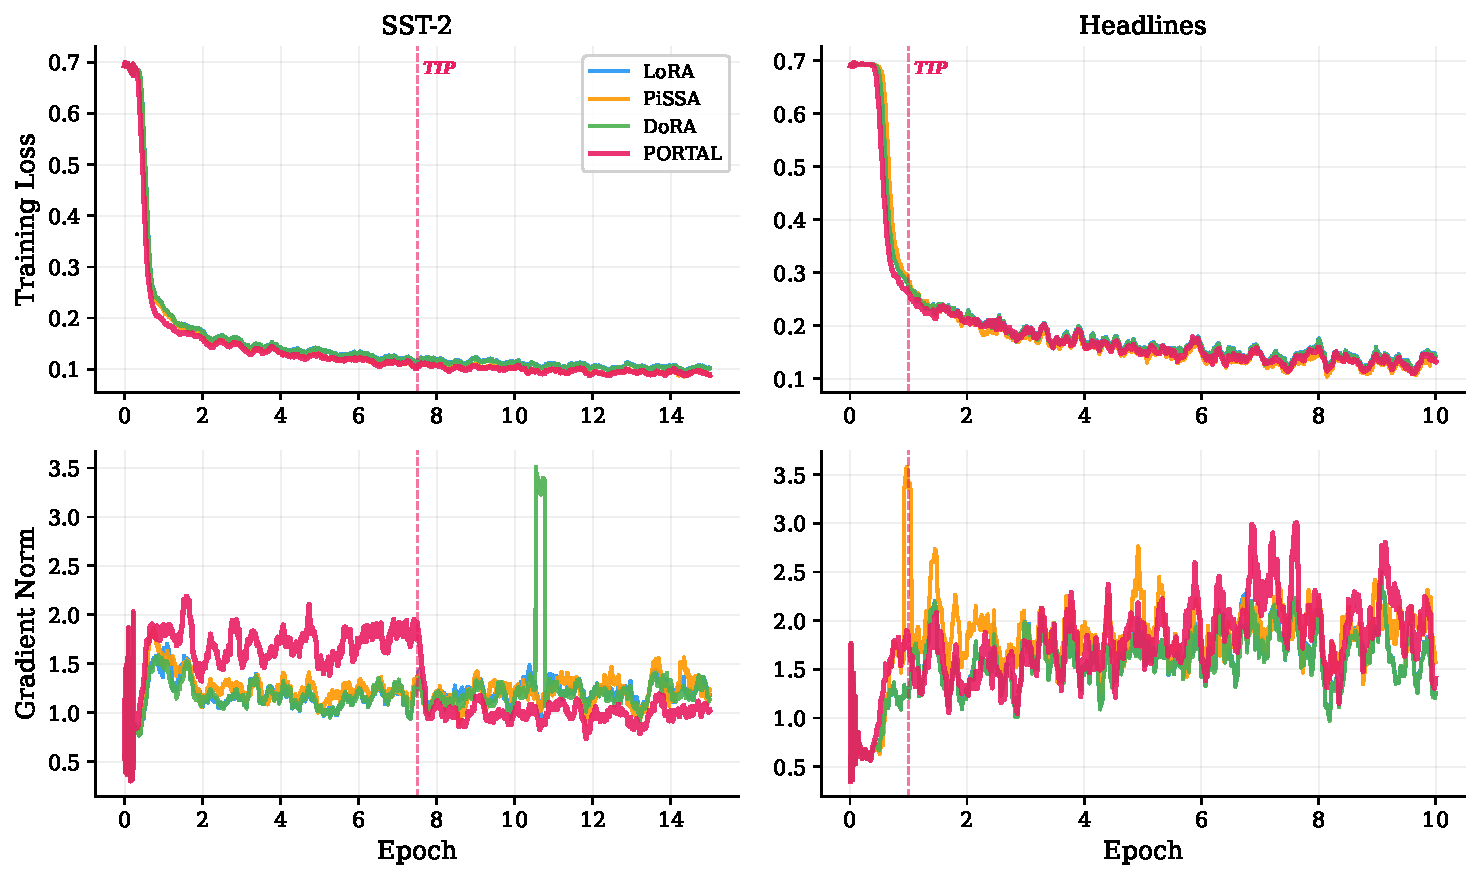
\includegraphics[width=\textwidth]{figures/fig_training_method_comparison.pdf}
\caption{Training loss and gradient norm on representative NLU and sarcasm runs.
The switch event introduces no visible loss jump, consistent with the loss-preserving projection in Eq.~\ref{eq:equivalence}.}
\label{fig:method_comparison}
\end{figure}

\begin{figure}[!ht]
\centering
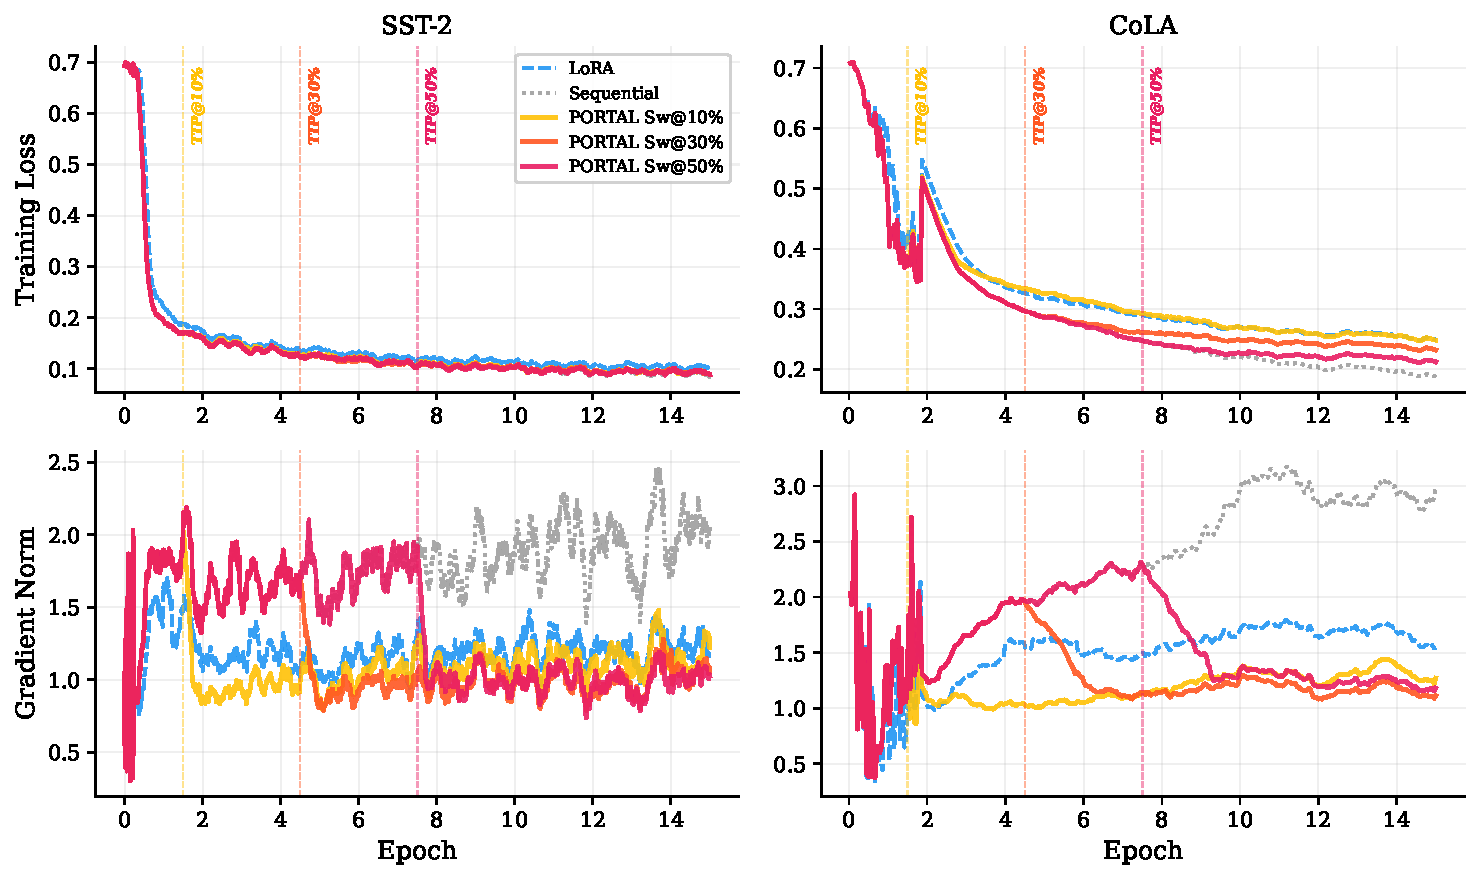
\includegraphics[width=\textwidth]{figures/fig_training_switch_comparison.pdf}
\caption{Effect of switching-point choice on training dynamics.
Earlier switching follows LoRA-like behavior; later switching retains longer sequential probing and can improve hard tasks.}
\label{fig:switch_comparison}
\end{figure}

%=============================================================================
\newpage
\section*{NeurIPS Paper Checklist}

\begin{enumerate}

\item {\bf Claims}
    \item[] Question: Do the main claims made in the abstract and introduction accurately reflect the paper's contributions and scope?
    \item[] Answer: \answerYes{}
    \item[] Justification: The abstract and introduction clearly state four contributions (time-axis generalization, task-aware convergence, ultra-fast SVD, zero inference latency) that are supported by the theoretical analysis in Section~3 and experiments in Section~4.

\item {\bf Limitations}
    \item[] Question: Does the paper discuss the limitations of the work performed by the authors?
    \item[] Answer: \answerYes{}
    \item[] Justification: Section~6 (Conclusion) includes a dedicated limitations paragraph discussing the need for validation-based $T_{\mathrm{switch}}$ selection and the scope of experiments (up to 7B parameters).

\item {\bf Theory assumptions and proofs}
    \item[] Question: For each theoretical result, does the paper provide the full set of assumptions and a complete (and correct) proof?
    \item[] Answer: \answerYes{}
    \item[] Justification: Theorems~1--4 and Propositions~1--2 include complete proofs in the main text (Section~3) and Appendix~A.

    \item {\bf Experimental result reproducibility}
    \item[] Question: Does the paper fully disclose all the information needed to reproduce the main experimental results of the paper to the extent that it affects the main claims and/or conclusions of the paper (regardless of whether the code and data are provided or not)?
    \item[] Answer: \answerYes{}
    \item[] Justification: Section~4.1 and Appendix~B provide complete hyperparameters, model specifications, dataset details, and evaluation protocols for all experiments.


\item {\bf Open access to data and code}
    \item[] Question: Does the paper provide open access to the data and code, with sufficient instructions to faithfully reproduce the main experimental results, as described in supplemental material?
    \item[] Answer: \answerNo{}
    \item[] Justification: Code will be released upon acceptance. All datasets used are publicly available and cited in the paper.


\item {\bf Experimental setting/details}
    \item[] Question: Does the paper specify all the training and test details (e.g., data splits, hyperparameters, how they were chosen, type of optimizer) necessary to understand the results?
    \item[] Answer: \answerYes{}
    \item[] Justification: Full training details including optimizer, learning rate, batch size, schedule, and evaluation protocols are provided in Section~4.1 and Appendix~B.

\item {\bf Experiment statistical significance}
    \item[] Question: Does the paper report error bars suitably and correctly defined or other appropriate information about the statistical significance of the experiments?
    \item[] Answer: \answerNo{}
    \item[] Justification: Due to the high computational cost of LLM fine-tuning experiments, we report single-run results following the standard protocol of prior work (LoRA, PiSSA). DeBERTa experiments were run with consistent seeds for fair comparison.

\item {\bf Experiments compute resources}
    \item[] Question: For each experiment, does the paper provide sufficient information on the computer resources (type of compute workers, memory, time of execution) needed to reproduce the experiments?
    \item[] Answer: \answerYes{}
    \item[] Justification: Section~4.1 specifies the models and precision settings. Appendix~B provides extended computational details.

\item {\bf Code of ethics}
    \item[] Question: Does the research conducted in the paper conform, in every respect, with the NeurIPS Code of Ethics \url{https://neurips.cc/public/EthicsGuidelines}?
    \item[] Answer: \answerYes{}
    \item[] Justification: This work proposes a general-purpose training methodology for parameter-efficient fine-tuning and does not raise specific ethical concerns.


\item {\bf Broader impacts}
    \item[] Question: Does the paper discuss both potential positive societal impacts and negative societal impacts of the work performed?
    \item[] Answer: \answerYes{}
    \item[] Justification: Section~6 discusses broader impact, noting that JELLY reduces computational barriers to fine-tuning while acknowledging that output quality depends on training data.

\item {\bf Safeguards}
    \item[] Question: Does the paper describe safeguards that have been put in place for responsible release of data or models that have a high risk for misuse (e.g., pre-trained language models, image generators, or scraped datasets)?
    \item[] Answer: \answerNA{}
    \item[] Justification: This paper proposes a training methodology and does not release pretrained models or datasets.

\item {\bf Licenses for existing assets}
    \item[] Question: Are the creators or original owners of assets (e.g., code, data, models), used in the paper, properly credited and are the license and terms of use explicitly mentioned and properly respected?
    \item[] Answer: \answerYes{}
    \item[] Justification: All datasets, models, and baselines are properly cited throughout the paper.

\item {\bf New assets}
    \item[] Question: Are new assets introduced in the paper well documented and is the documentation provided alongside the assets?
    \item[] Answer: \answerNA{}
    \item[] Justification: No new datasets or pretrained models are released. Code will be documented and released upon acceptance.

\item {\bf Crowdsourcing and research with human subjects}
    \item[] Question: For crowdsourcing experiments and research with human subjects, does the paper include the full text of instructions given to participants and screenshots, if applicable, as well as details about compensation (if any)?
    \item[] Answer: \answerNA{}
    \item[] Justification: This paper does not involve crowdsourcing or human subjects research.

\item {\bf Institutional review board (IRB) approvals or equivalent for research with human subjects}
    \item[] Question: Does the paper describe potential risks incurred by study participants, whether such risks were disclosed to the subjects, and whether Institutional Review Board (IRB) approvals (or an equivalent approval/review based on the requirements of your country or institution) were obtained?
    \item[] Answer: \answerNA{}
    \item[] Justification: This paper does not involve human subjects research.

\item {\bf Declaration of LLM usage}
    \item[] Question: Does the paper describe the usage of LLMs if it is an important, original, or non-standard component of the core methods in this research? Note that if the LLM is used only for writing, editing, or formatting purposes and does \emph{not} impact the core methodology, scientific rigor, or originality of the research, declaration is not required.
    \item[] Answer: \answerNA{}
    \item[] Justification: LLMs are not used as a component of the core methodology. LLMs (LLaMA-2-7B) are used as the subject of fine-tuning experiments, which is standard practice. GPT-4 is used as a judge for MT-Bench evaluation following the established protocol.

\end{enumerate}


\end{document}
